\documentclass[final, 20pt]{beamer}
% poster
\usepackage[size=custom, width=121.92, height=91.44]{beamerposter}
% common stuff
\usepackage{graphicx}
\usepackage{hyperref}
\usepackage{booktabs}
\usepackage{amsmath}
\usepackage{caption}
\usepackage{subcaption}
\usepackage{enumitem}
\usepackage{array}
\usepackage{xparse}
\usepackage{wrapfig}
\usepackage{xspace}
% necessary acronyms
\def\ie{\textit{i.e.}\xspace}
\def\eg{\textit{e.g.}\xspace}
\def\etc{\textit{etc.}\xspace}
\def\etal{\textit{et al.}\xspace}
\def\cf{\textit{cf.}\xspace}
% font
\usefonttheme{serif}
\setbeamerfont{block title}{size=\Large, series=\bfseries}
\setbeamerfont{headline title}{size=\fontsize{96}{0pt}\selectfont, series=\bfseries}
\setbeamerfont{headline author}{size=\large, series=\bfseries}
% main color
\definecolor{theme-1}{HTML}{3b82f6} % #3b82f6
\definecolor{theme-2}{HTML}{0AA1DD} % #0AA1DD
\definecolor{theme-3}{HTML}{79DAE8} % #79DAE8
\definecolor{theme-4}{HTML}{E8F9FD} % #E8F9FD
% set color
\setbeamercolor{block title}{fg=white, bg=theme-2}
\setbeamercolor{headline title}{fg=white, fg=theme-2}
% linespace
\usepackage{setspace}
\setstretch{1.5}
% size
\setlength{\paperwidth}{48in}
\setlength{\paperheight}{36in}
\newlength{\sepwidth}
\newlength{\colwidth}
\newlength{\twocolwidth}
\newlength{\contentwidth}
\newlength{\contentheight}
\newlength{\marginwidth}

\usepackage{calc}
\setlength{\marginwidth}{1in}
\setlength{\contentwidth}{\paperwidth - 2\marginwidth}
\setlength{\contentheight}{\paperheight - 3in}
\setlength{\sepwidth}{0.005\contentwidth}
% 4 columns
\setlength{\colwidth}{(\contentwidth - 2\sepwidth) / 3}
\setlength{\twocolwidth}{\colwidth + \sepwidth + \colwidth}
% empty spacer column
\NewDocumentCommand{\separatorcolumn}{}{\begin{column}{\sepwidth}\end{column}}
\NewDocumentCommand{\margincolumn}{}{\begin{column}{\marginwidth}\end{column}}
% top head template
\setbeamertemplate{headline}{
  \begin{beamercolorbox}{headline}
    \usebeamerfont{headline}
    \vskip1.5in
    \centering
    {\usebeamerfont{headline title}\usebeamercolor[fg]{headline title}\inserttitle\\[0.5ex]}
    {\usebeamerfont{headline author}\usebeamercolor[fg]{headline author}\insertauthor\\[1ex]} % author is not allowed.
    \ifbeamercolorempty[bg]{headline rule}{}{
      \begin{beamercolorbox}[wd=\paperwidth,colsep=0.5ex]{headline rule}\end{beamercolorbox}
    }
  \end{beamercolorbox}
}
\usepackage{tikz}
\usetikzlibrary{calc}
\NewDocumentCommand{\ensuremargin}{}{
  \begin{tikzpicture}[remember picture,overlay]
    \draw[black] ($(current page.north west) - (0, 1.5in)$) -- ($(current page.north east) - (0, 1.5in)$);
    \draw[black] ($(current page.south west) + (0, 1.5in)$) -- ($(current page.south east) + (0, 1.5in)$);
    \draw[black] ($(current page.north west) + (1in, 0)$) -- ($(current page.south west) + (1in, 0)$);
    \draw[black] ($(current page.north east) - (1in, 0)$) -- ($(current page.south east) - (1in, 0)$);
  \end{tikzpicture}
}
% header helper
\usepackage{xhfill}
\NewDocumentCommand{\header}{m O{1.5em}}{\vspace{#2}\begingroup\usebeamercolor[bg]{block title}\scshape\large#1\par\vspace{-0.55\baselineskip}\hrulefill\endgroup}
\NewDocumentCommand{\subheader}{m}{\begingroup\usebeamercolor[bg]{block title}\bfseries#1\par\endgroup}

% multicol
\usepackage{multicol}
% hanging indent
\usepackage{hanging}
% color
\setbeamercolor{block title}{fg=white, bg=theme-2}
% numbered figure and table
\setbeamertemplate{caption}[numbered]
% metadata
\title{Wireless Online Real-time Language Expression Yielder}
\author{Ian Oberbeck \& Yubo Cao \& Anish Goyal \\\normalfont\selectfont GOSA Governor's Honors Program 60 Engineering}
% bullet
\setlist[itemize]{leftmargin=0.5em, label=\usebeamercolor[bg]{block title}\textbullet}
% redefine block
\let\block=\undefined
\let\endblock=\undefined
\usepackage[most]{tcolorbox}
\newtcolorbox{block}[1]{enhanced, colback=white, colframe=theme-2!50, colbacktitle=theme-2, coltitle=white, fonttitle=\bfseries, title=\Large#1, boxrule=1pt, boxsep=1.5em, breakable, sharpish corners, bottomrule=0.5em, toptitle=-0.75em, bottomtitle=-0.75em}
% microtype
\usepackage[activate={true,nocompatibility},final]{microtype}

% remove navigation
\setbeamertemplate{navigation symbols}{}
% make vfill work in beamer columns
\usepackage{etoolbox}
\let\oldcolumn\column
\let\oldendcolumn\endcolumn
\RenewDocumentEnvironment{column}{m O{\contentheight - 2.7in}}{%
  \oldcolumn{#1}%
  \minipage[c][#2][s]{\columnwidth}
}{\endminipage\oldendcolumn}

\begin{document}

\begin{frame}[t]
  \centering
  \begin{columns}[t]
    \margincolumn

    \begin{column}{\colwidth}
      \begin{block}{Mechanical Design}
        \header{Cord Actuation}[0pt]

        \begin{wrapfigure}{r}{0.35\linewidth}
          \centering
          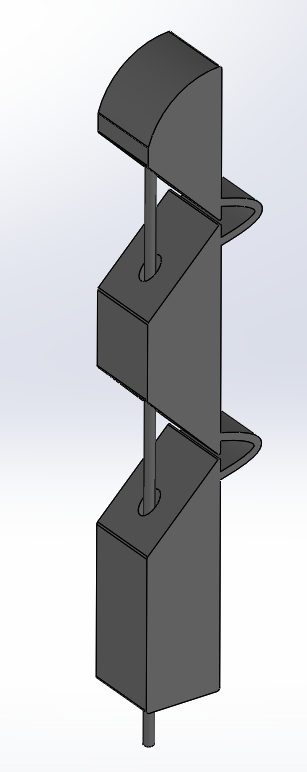
\includegraphics[width=0.35\linewidth]{images/finger.png}
          \caption{CAD of cord actuation design}
          \label{fig:cord-actuation}
        \end{wrapfigure}

        The fingers are curled by servo-driven pull cords. By reducing the available length of the cord, the surfaces of the finger segments are pulled closer to one another. The surfaces are angled 90 degrees; so the finger rotates around the back (where there is no gap) to curl. We utilized ripoff SG90 servos for this task, as they're cost-effective, space-efficient, and have the minimum sufficient torque required to actuate the fingers.

        \header{Compliant Hinges}[2cm]

        \begin{wrapfigure}{r}{0.35\linewidth}
          \centering
          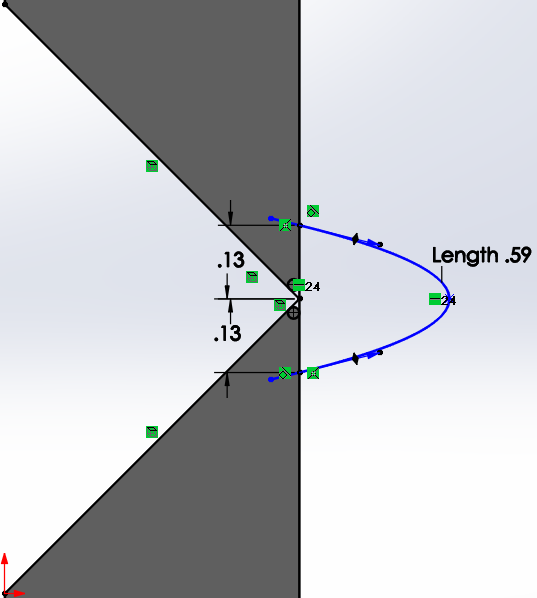
\includegraphics[width=0.75\linewidth]{images/compliant-hinge.png}
          \caption{CAD of compliant hinge design}
          \label{fig:compliant-hinge}
        \end{wrapfigure}

        Compliant hinges connect the finger segments, allowing the finger to curl as a single part. This is accomplished by 3D printing the fingers in polypropylene (PP); a polymer ideally suited for compliant hinges due to its fatigue-resistant and semi-rigid properties. The hinges are designed using splines constrained by their connection points and length, such that when the segment is rotated 90 degrees it has the proper length to temporarily deform into a circle. The energy stored in this deformation allows the fingers to passively return to their original position when the cord tension is released.
      \end{block}

      \begin{block}{Material}
        \begin{itemize}
          \item 5 SG90 servo, servo horns, and screws
          \item 4 3D printed fingers + 1 3D printed palm
          \item Polypropylene filament \& Polylactic acid filament
          \item 1 Raspberry PI 4B
          \item \texttt{faster\_whisper}, \texttt{pytorch}, \texttt{asyncio}, \texttt{pyav}, \texttt{aiohttp}, \texttt{aiortc}, Expo Framework.
        \end{itemize}
      \end{block}


    \end{column}

    \separatorcolumn

    \begin{column}{\colwidth}
      \begin{block}{Goal}

        The goal of \textsc{Project Worley} is to create a wireless online real-time language expression yielder (WORLEY) that can be used to act out American Sign Language (ASL) in real-time. Specifically, WORLEY will be able to:

        \begin{itemize}
          \item Recognize speech and translate it into ASL in real-time.
          \item Act out the translation on the robotic hand through remote general-purpose input/output (GPIO) control.
        \end{itemize}

        \header{Motivation}[0pt]

        Our friend Cory suffered from hearing loss, making communication difficult. We aimed to develop a device to improve communication and quality of life for Cory and others in similar situations.

        This device can also be used for Pre-K and K-12 students.  While it may seem easy for parents to learn ASL and teach it to their kids, ASL is a complex language with its grammar, syntax, and nuances. \emph{WORLEY} give necessary language exposure \& support for the deaf children and their parents.
      \end{block}

      \begin{block}{Significance}
        \header{Existing Solution}[0pt]

        \begin{figure}[ht]
          \centering
          \begin{subfigure}[b]{0.45\linewidth}
            \centering
            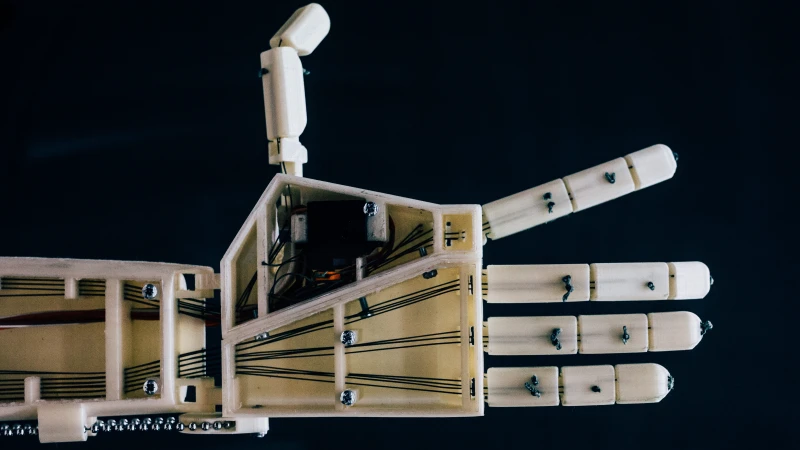
\includegraphics[width=\linewidth]{images/aslan.png}
            \caption{Project ASLAN}
            \label{fig:aslan}
          \end{subfigure}
          \begin{subfigure}[b]{0.45\linewidth}
            \centering
            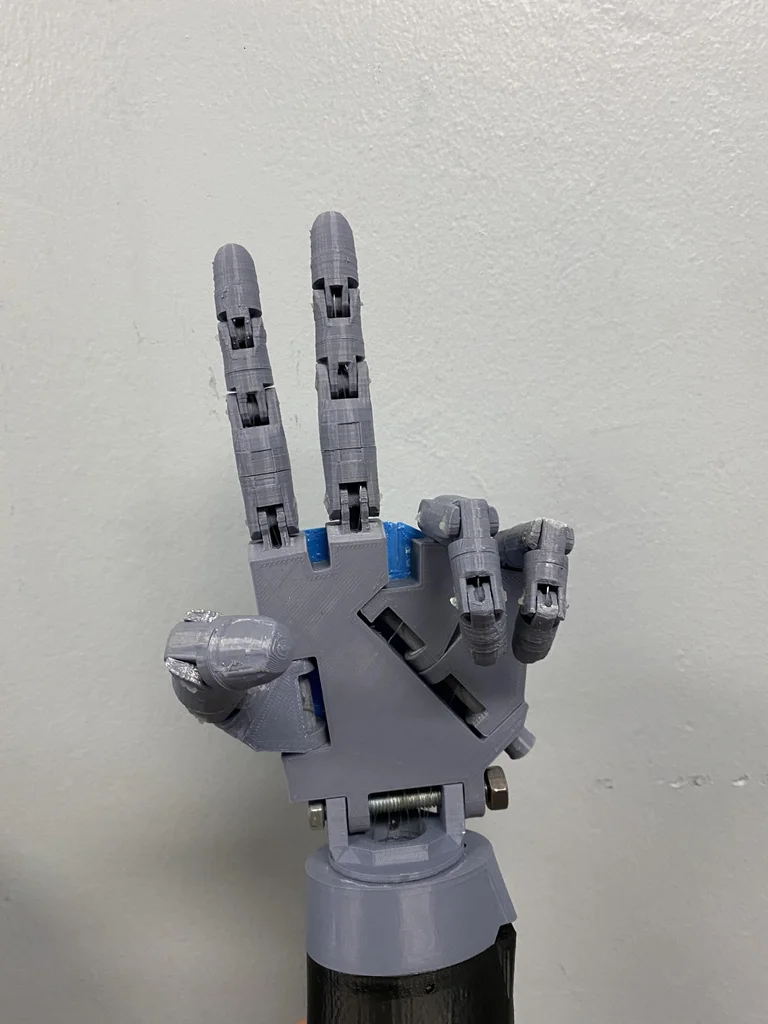
\includegraphics[width=0.425\linewidth]{images/instructable-hand.png}
            \caption{Instructable Hand}
            \label{fig:instructable-hand}
          \end{subfigure}
        \end{figure}

        Existing solutions to act out ASL exists. However, they have several drawbacks:

        \begin{itemize}
          \item They merely perform manually-coded English (MCE), which is not the same as ASL and doesn't have the same grammar, syntax, and nuances.
          \item They are incapable to act out ASL in real-time or require text input instead of speech input.
        \end{itemize}

        \header{Significance}[2cm]

        \begin{itemize}
          \item 10,000 people in the United States are registered as ASL interpreters.
          \item In comparison, 37.5 million people in the United States suffer from hearing problems.
          \item ASL is the third most used language in the United States \& the Americans with Disabilities Act (ADA) requires businesses to provide ASL interpreters.
          \item In the United States, 30 deaf children are born every day, and 90\% of their parents do not know ASL.
          \item \emph{WORLEY} will help to solve this problem by providing a low-cost, portable, and easy-to-use solution for ASL interpretation.
        \end{itemize}
      \end{block}
    \end{column}

    \separatorcolumn

    \begin{column}{\colwidth}
      \begin{block}{System Architeture}
        \begin{figure}[ht]
          \centering
          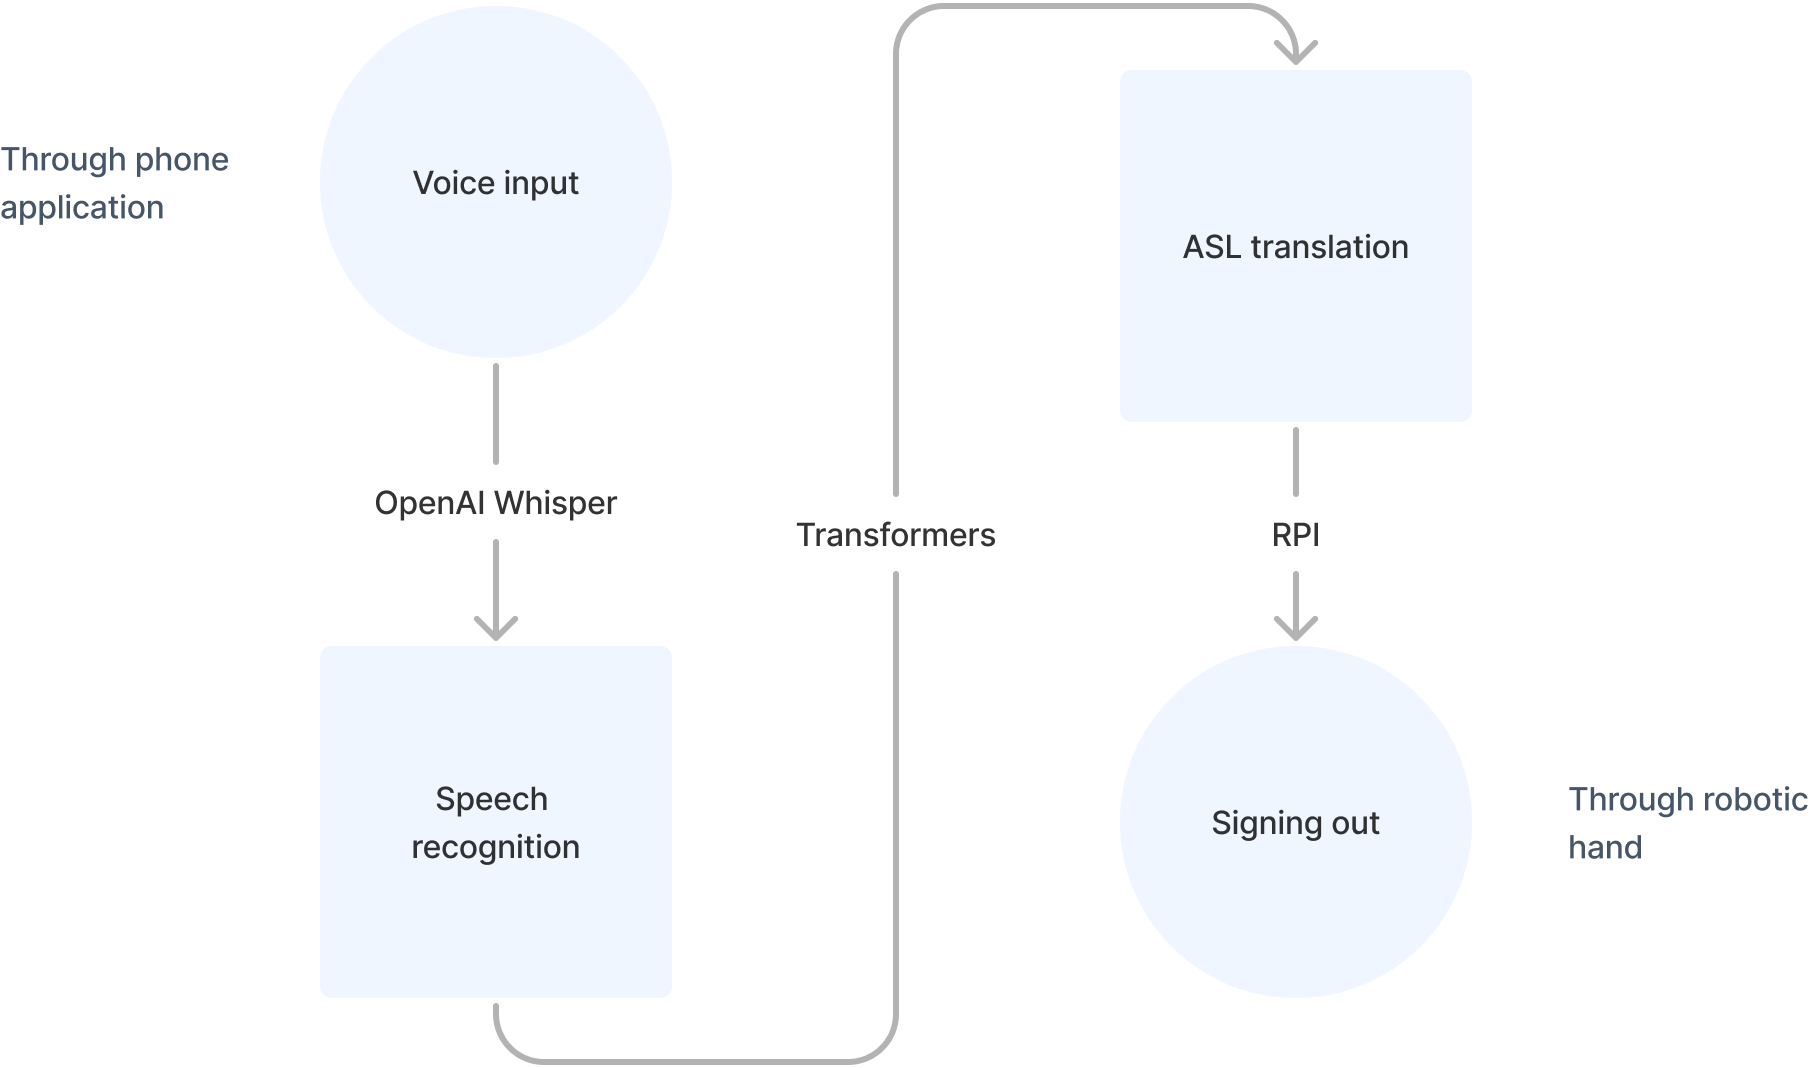
\includegraphics[width=0.85\linewidth]{images/flowchart.png}
          \caption{Flowchart of the system architecture}
          \label{fig:flowchart}
        \end{figure}

        \begin{itemize}
          \item The user speaks into the Worley application on their phone.
          \item The application establishes a Web real-time communication (WebRTC) connection with the server and streams the audio.
          \item The server runs a lightweight voice activation detection (VAD) model \texttt{sliero} detects speech. Such results are buffered into a queue along with the timestamps, and a 2-pointer technique is used to extract the longest continuous subsequence, \ie, the speech. Such segments are sent to \texttt{whisper} for speech recognition.
          \item The text is translated to ASL language using a custom-built transformer model trained on the \texttt{ASLG-PC12} dataset.
          \item The ASL translation is sent to the Raspberry Pi, which controls the robotic hand, and the mobile application.
        \end{itemize}
      \end{block}

      \begin{block}{Challenges}
        \begin{itemize}
          \item More tolerance would be needed for the servo motors to control the index finger to move behind the palm.
          \item Whisper model, even the CTranslate2 version, would require $1735\,\text{ms}\pm 139\,\text{ms}$ to translate a 3-second speech, which is not real-time. Deployment of the servo independently from the HTTP server on KServe would be needed to ensure performance and scalability.
          \item Polypropylene failed to print successfully on the 3D printer; further, the printed version has structural defects \& fatigue issues, rendering the hand to be less realistic.
        \end{itemize}
      \end{block}

      \begin{block}{Conclusions}
        In this project, we successfully developed a robotic hand that can act out ASL and be controlled using a mobile application and voice commands.

        Despite defects in the final product, along with many challenges that we faced on the road, we believe that this project has the potential to be further developed and improved. Future work could focus on improving the performance and scalability of the speech recognition system, as well as enhancing the realism of the hand. Overall, this project demonstrates the potential of combining robotics, mobile applications, and speech recognition to create innovative and interactive systems.
      \end{block}
    \end{column}

    \margincolumn
  \end{columns}

  \tikz {
    \draw ($(current page.south west)!0.5!(current page.south east)$) node {All charts, graphs, photos, and diagrams are the product of the student researcher.};
  }
\end{frame}
\end{document}

